\documentclass{article}

\usepackage{../mathclub}

\DeclareMathOperator{\Conf}{Conf}
\DeclareMathOperator{\MCG}{MCG}

\title{Braids and Configuration Spaces} 
\author{}
\date{February 22, 2022}

\begin{document}

\section{Introduction}

Welcome to Math Club week 8! Today, we will take a look at braids and configuration spaces. The history of braids begins thousands of years ago, and they entered the realm of mathematics at least several centuries ago. The modern mathematical study of braids involves lots of beautiful geometry and group theory. Compared to braids, configuration spaces tend to be more mysterious in the sense that a configuration space of a general topological space can be quite complicated (with hard-to-compute homology/cohomology). 

This is an active area of research that combines tools from classical topology, quantum topology, representation theory, and physics. Some major achievements include the colored Jones representations and Lawrence-Krammer-Bigelow representations of Braid groups. 

Most of the content below are drawn from Prof. Zhenghan Wang's Math 227B and Chapter 18 of ``Office Hours with a Geometric Group Theorist.'' While some exercises below are doable, others might be very hard, so take it easy if you get stuck.   
\section{Preliminaries}  

\subsection{Braids and braid groups} 

\begin{definition}
Informally speaking, a $n$-string braid consists of $n$ strings which cross each other a finite number of times, do not intersect with themselves or any of the other strands, and travel strictly from left wall to right wall. 
\end{definition}

\begin{figure}[hbt!]
\label{fig:aa}
\small
\centering
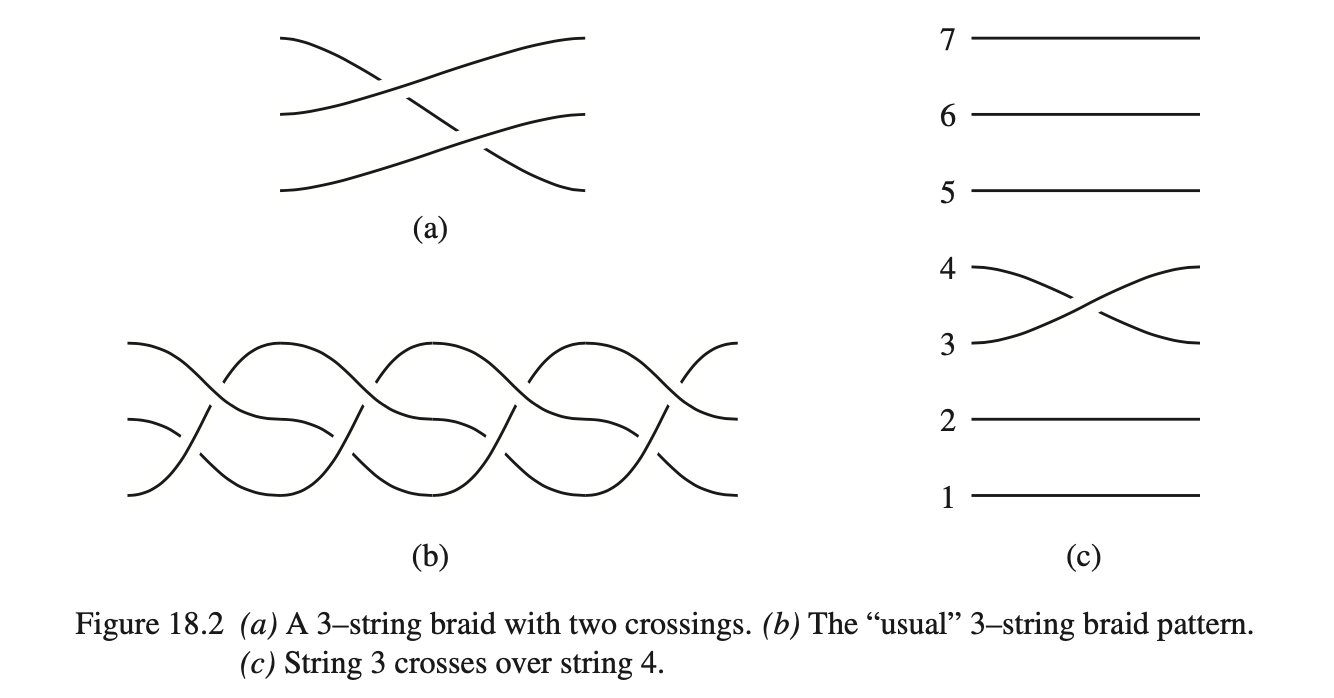
\includegraphics[scale = 0.5]{Pics/2.png}
\end{figure}
\leavevmode

\begin{definition}
Informally speaking, two braids are defined equivalent if you can move one braid, keeping it between the walls and keeping the endpoints fixed, and make it look like the other. 
\end{definition}

This defines an equivalence relation on all $n$-string braids. One can check that for fixed $n$, the equivalence classes of $n$-string braids form a group. This group is called the $n$-string braid group. The picture on next page illuminates on the proof. 
\begin{figure}[hbt!]
\label{fig:bb}
\small
\centering
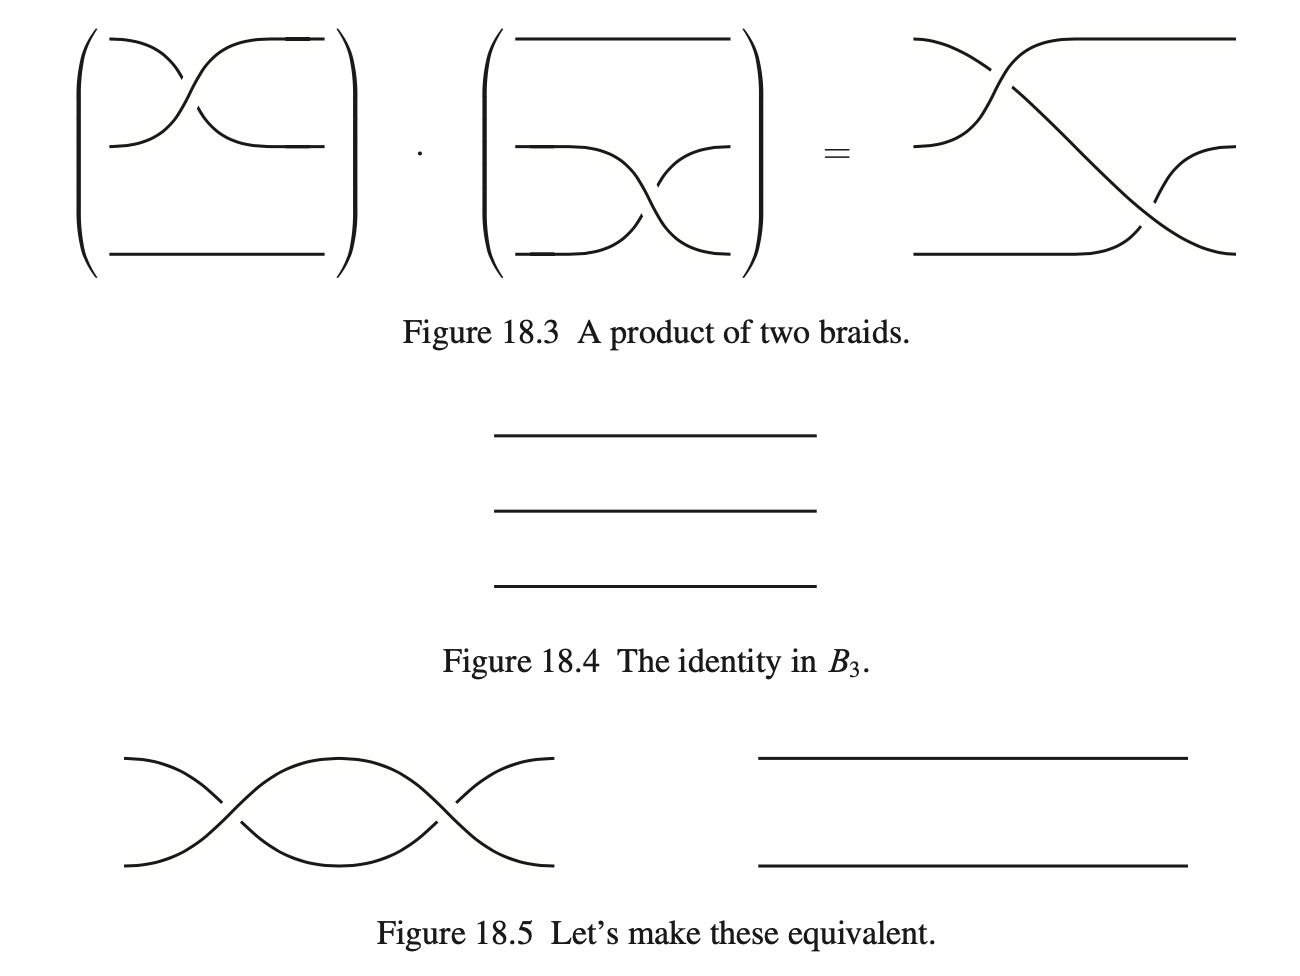
\includegraphics[scale = 0.5]{Pics/3.png}
\end{figure}
\leavevmode

\begin{definition}
The $n$-string braid group has the presentation
\[
B_{n} = \langle \sigma_{1}, \ldots, \sigma_{n - 1}| \sigma_{i} \sigma_{j} = \sigma_{j} \sigma_{i} \text{ for $|i - j| > 1$}, \sigma_{i} \sigma_{i + 1} \sigma_{i} = \sigma_{i + 1} \sigma_{i} \sigma_{i + 1} \text{ for $1 \leq i \leq n - 2$} 
\rangle.
\]
\end{definition}

There's a map $\pi: B_{n} \rightarrow S_{n}$ where you take a braid, ignore the overs and unders, and just read the corresponding permutation. One can check that $\pi$ is a group homomorphism. 
 
\begin{definition}
The kernel of the map $\pi: B_{n} \rightarrow S_{n}$ is called the pure braid group $PB_{n}$. It consists of all braids in $B_{n}$ such that the strings line up in the same order on the left as they do on the right.
\end{definition}

There are various ways of obtaining $B_{n}$. We mention three of them:
\begin{itemize}
    \item Artin braid diagram 
    \item $B_{n}$ as the mapping class group of $n$-punctured disk 
    \item $B_{n}$ as the fundamental group of $n$-th unordered configuration space of $\mathbb{R}^{2}$ 
\end{itemize}
The definition of a mapping class group is given below while the definition of a configuration space is postponed to next subsection.

\begin{definition}
Given $M$ a topological manifold, we define the mapping class group of $M$ to be the group of isotopy classes of homeomorphisms of $M$, denoted by $\MCG(M)$. 
\end{definition}

\begin{figure}[hbt!]
\label{fig:cc}
\small
\centering
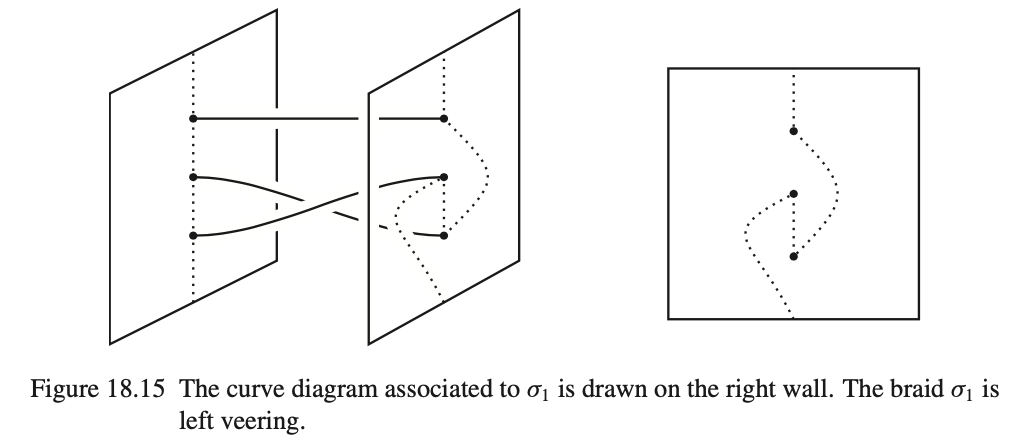
\includegraphics[scale = 0.6]{Pics/4.png}
\end{figure}
\leavevmode

\subsection{Configuration spaces}

\begin{definition}
For a topological space $Y$, the $n$-th ordered configuration space of $Y$ is the set of $n$-tuples of pairwise distinct points in $Y$: 
\[
\Conf_{n}(Y) := \{(y_{1}, \ldots, y_{n}) \in Y^{n}| y_{i} \neq y_{j} \text{ for $i \neq j$}\}.  
\]
\end{definition}

\begin{definition}
There's a natural action of the symmetric group $S_{n}$ on the points in $\Conf_{n}(Y)$. This action gives rise to the $n$-th unordered configuration space of $Y$: 
\[
\Conf^{S}_{n}(Y) := \Conf_{n}(Y)/S_{n}.   
\]
\end{definition}

\section{Exercises}

\begin{exercise}
Assure yourself that $B_{1} = \{0\}$, $B_{2} \cong \mathbb{Z}$, and $B_{3} = \langle \sigma_{1}, \sigma_{2}| \sigma_{1} \sigma_{2} \sigma_{1} = \sigma_{2} \sigma_{1} \sigma_{2} \rangle$. 
\end{exercise}

\begin{exercise}
By defining a map from $\langle x, y |x^{3} = y^{2} \rangle$ to $B_{3}$ that sends $x$ to $\sigma_{1} \sigma_{2}$ and $y$ to $\sigma_{1} \sigma_{2} \sigma_{1}$, prove that 
\[B_{3} \cong \langle x, y |x^{3} = y^{2} \rangle.\]
\end{exercise}

\begin{exercise}
Show that the abelianization of $B_{n}$ is isomorphic to $\mathbb{Z}$ when $n \geq 2$ (hint: observe that all generators $\sigma_{i}$ are conjugate to each other).  
\end{exercise}

\begin{exercise}
Let $Y$ be a topological space. Assure yourself that 
\[
\Conf_{1}(Y) = Y \text{ and } \Conf_{2}(Y) = Y \times Y - \Delta, 
\]
where $\Delta$ is the diagonal of $Y \times Y$. In particular, when $Y = S^{1}$, show that 
$\Conf_{2}^{S}(S^{1})$ is homeomorphic to an open M\"{o}bius band.  
\end{exercise}

\begin{exercise}
Prove that $\Conf_{2}(\mathbb{R}^{n})$ is homotopy equivalent to $S^{n - 1}$ by constructing a homeomorphism (the Gauss map) from $\Conf_{2}(\mathbb{R}^{n})$ to $S^{n - 1} \times \mathbb{R}_{>0} \times \mathbb{R}^{n}$. 
\end{exercise}

\begin{exercise}
Show that $\Conf_{n}(\mathbb{R}^{2})$ is an Eilenberg-Maclane space of type $K(\pi, 1)$, i.e. all higher-order homotopy groups vanish except for the fundamental group.  
\end{exercise}

\begin{exercise}
Show that $\Conf_{2}^{S}(S^{1})$ is homotopy equivalent to $S^{1}$. In general, one can check that $\Conf_{n}^{S}(S^{1})$ is homotopy equivalent to $S^{1}$.    
\end{exercise}

\begin{exercise}
Verify that Lens spaces $L(7, 1)$ and $L(7, 2)$ have different configuration spaces. Deduce that the configuration space is not a homotopy invariant. 
\end{exercise}

\begin{exercise} 
Recall the definitions of braid group and pure braid group. Verify that 
\[
B_{n} \cong \pi_{1}(\Conf^{S}_{n}(\mathbb{R}^{2})) \text{ and } PB_{n} \cong \pi_{1}(\Conf_{n}(\mathbb{R}^{2})). 
\]
\end{exercise}

\section{Algebraic Machinery}
We list some useful machinery from algebraic topology that are used to compute the homotopy/homology/cohomology of the configuration spaces: 
\begin{itemize}
    \item Fadell-Neuwirth fibration theorem
    \item Serre fibration theorem 
    \item Serre spectral sequence 
    \item Leray-Hirsch theorem
    \item Poincare polynomial 
\end{itemize}
We're not going to discuss them in any details. Explore them if you feel interested and have time! 
\end{document}